

\tikzset{every picture/.style={line width=0.75pt}} %set default line width to 0.75pt        

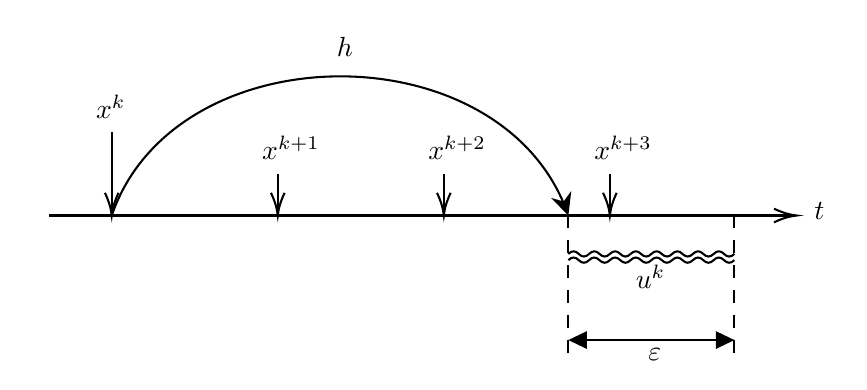
\begin{tikzpicture}[x=0.75pt,y=0.75pt,yscale=-1,xscale=1]
%uncomment if require: \path (0,300); %set diagram left start at 0, and has height of 300

%Straight Lines [id:da38129597128288384] 
\draw    (10,90) -- (368,90) ;
\draw [shift={(370,90)}, rotate = 180] [color={rgb, 255:red, 0; green, 0; blue, 0 }  ][line width=0.75]    (10.93,-3.29) .. controls (6.95,-1.4) and (3.31,-0.3) .. (0,0) .. controls (3.31,0.3) and (6.95,1.4) .. (10.93,3.29)   ;
%Straight Lines [id:da3970383883562073] 
\draw    (40,50) -- (40,88) ;
\draw [shift={(40,90)}, rotate = 270] [color={rgb, 255:red, 0; green, 0; blue, 0 }  ][line width=0.75]    (10.93,-3.29) .. controls (6.95,-1.4) and (3.31,-0.3) .. (0,0) .. controls (3.31,0.3) and (6.95,1.4) .. (10.93,3.29)   ;
%Straight Lines [id:da569816085224214] 
\draw    (120,70) -- (120,88) ;
\draw [shift={(120,90)}, rotate = 270] [color={rgb, 255:red, 0; green, 0; blue, 0 }  ][line width=0.75]    (10.93,-3.29) .. controls (6.95,-1.4) and (3.31,-0.3) .. (0,0) .. controls (3.31,0.3) and (6.95,1.4) .. (10.93,3.29)   ;
%Straight Lines [id:da6348301753031073] 
\draw    (200,70) -- (200,88) ;
\draw [shift={(200,90)}, rotate = 270] [color={rgb, 255:red, 0; green, 0; blue, 0 }  ][line width=0.75]    (10.93,-3.29) .. controls (6.95,-1.4) and (3.31,-0.3) .. (0,0) .. controls (3.31,0.3) and (6.95,1.4) .. (10.93,3.29)   ;
%Straight Lines [id:da13497978310705738] 
\draw    (280,70) -- (280,88) ;
\draw [shift={(280,90)}, rotate = 270] [color={rgb, 255:red, 0; green, 0; blue, 0 }  ][line width=0.75]    (10.93,-3.29) .. controls (6.95,-1.4) and (3.31,-0.3) .. (0,0) .. controls (3.31,0.3) and (6.95,1.4) .. (10.93,3.29)   ;
%Curve Lines [id:da7725246465957983] 
\draw    (40,90) .. controls (70.29,1.69) and (226.24,0.42) .. (259.04,87.34) ;
\draw [shift={(260,90)}, rotate = 251.14] [fill={rgb, 255:red, 0; green, 0; blue, 0 }  ][line width=0.08]  [draw opacity=0] (10.72,-5.15) -- (0,0) -- (10.72,5.15) -- (7.12,0) -- cycle    ;
%Straight Lines [id:da9656205587631153] 
\draw  [dash pattern={on 4.5pt off 4.5pt}]  (260,90) -- (260,160) ;
%Straight Lines [id:da8670670758401987] 
\draw  [dash pattern={on 4.5pt off 4.5pt}]  (340,90) -- (340,160) ;
%Straight Lines [id:da9146459318401605] 
\draw    (260,108.5) .. controls (261.67,106.83) and (263.33,106.83) .. (265,108.5) .. controls (266.67,110.17) and (268.33,110.17) .. (270,108.5) .. controls (271.67,106.83) and (273.33,106.83) .. (275,108.5) .. controls (276.67,110.17) and (278.33,110.17) .. (280,108.5) .. controls (281.67,106.83) and (283.33,106.83) .. (285,108.5) .. controls (286.67,110.17) and (288.33,110.17) .. (290,108.5) .. controls (291.67,106.83) and (293.33,106.83) .. (295,108.5) .. controls (296.67,110.17) and (298.33,110.17) .. (300,108.5) .. controls (301.67,106.83) and (303.33,106.83) .. (305,108.5) .. controls (306.67,110.17) and (308.33,110.17) .. (310,108.5) .. controls (311.67,106.83) and (313.33,106.83) .. (315,108.5) .. controls (316.67,110.17) and (318.33,110.17) .. (320,108.5) .. controls (321.67,106.83) and (323.33,106.83) .. (325,108.5) .. controls (326.67,110.17) and (328.33,110.17) .. (330,108.5) .. controls (331.67,106.83) and (333.33,106.83) .. (335,108.5) .. controls (336.67,110.17) and (338.33,110.17) .. (340,108.5) -- (340,108.5)(260,111.5) .. controls (261.67,109.83) and (263.33,109.83) .. (265,111.5) .. controls (266.67,113.17) and (268.33,113.17) .. (270,111.5) .. controls (271.67,109.83) and (273.33,109.83) .. (275,111.5) .. controls (276.67,113.17) and (278.33,113.17) .. (280,111.5) .. controls (281.67,109.83) and (283.33,109.83) .. (285,111.5) .. controls (286.67,113.17) and (288.33,113.17) .. (290,111.5) .. controls (291.67,109.83) and (293.33,109.83) .. (295,111.5) .. controls (296.67,113.17) and (298.33,113.17) .. (300,111.5) .. controls (301.67,109.83) and (303.33,109.83) .. (305,111.5) .. controls (306.67,113.17) and (308.33,113.17) .. (310,111.5) .. controls (311.67,109.83) and (313.33,109.83) .. (315,111.5) .. controls (316.67,113.17) and (318.33,113.17) .. (320,111.5) .. controls (321.67,109.83) and (323.33,109.83) .. (325,111.5) .. controls (326.67,113.17) and (328.33,113.17) .. (330,111.5) .. controls (331.67,109.83) and (333.33,109.83) .. (335,111.5) .. controls (336.67,113.17) and (338.33,113.17) .. (340,111.5) -- (340,111.5) ;
%Straight Lines [id:da9421009511716788] 
\draw    (263,150) -- (337,150) ;
\draw [shift={(340,150)}, rotate = 180] [fill={rgb, 255:red, 0; green, 0; blue, 0 }  ][line width=0.08]  [draw opacity=0] (8.93,-4.29) -- (0,0) -- (8.93,4.29) -- cycle    ;
\draw [shift={(260,150)}, rotate = 0] [fill={rgb, 255:red, 0; green, 0; blue, 0 }  ][line width=0.08]  [draw opacity=0] (8.93,-4.29) -- (0,0) -- (8.93,4.29) -- cycle    ;
%Straight Lines [id:da08809531432681827] 
\draw [color={rgb, 255:red, 255; green, 255; blue, 255 }  ,draw opacity=1 ]   (0,0) -- (390,0) ;

% Text Node
\draw (377,82.4) node [anchor=north west][inner sep=0.75pt]    {$t$};
% Text Node
\draw (31,30.4) node [anchor=north west][inner sep=0.75pt]    {$x^{k}$};
% Text Node
\draw (111,50.4) node [anchor=north west][inner sep=0.75pt]    {$x^{k+1}$};
% Text Node
\draw (191,50.4) node [anchor=north west][inner sep=0.75pt]    {$x^{k+2}$};
% Text Node
\draw (11,52.4) node [anchor=north west][inner sep=0.75pt]    {$\dotsc $};
% Text Node
\draw (311,52.4) node [anchor=north west][inner sep=0.75pt]    {$\dotsc $};
% Text Node
\draw (271,50.4) node [anchor=north west][inner sep=0.75pt]    {$x^{k+3}$};
% Text Node
\draw (147,2.4) node [anchor=north west][inner sep=0.75pt]    {$h$};
% Text Node
\draw (291,112.4) node [anchor=north west][inner sep=0.75pt]    {$u^{k}$};
% Text Node
\draw (297,152.4) node [anchor=north west][inner sep=0.75pt]    {$\varepsilon $};


\end{tikzpicture}
